\subsection*{Partie A}
	\begin{center}
		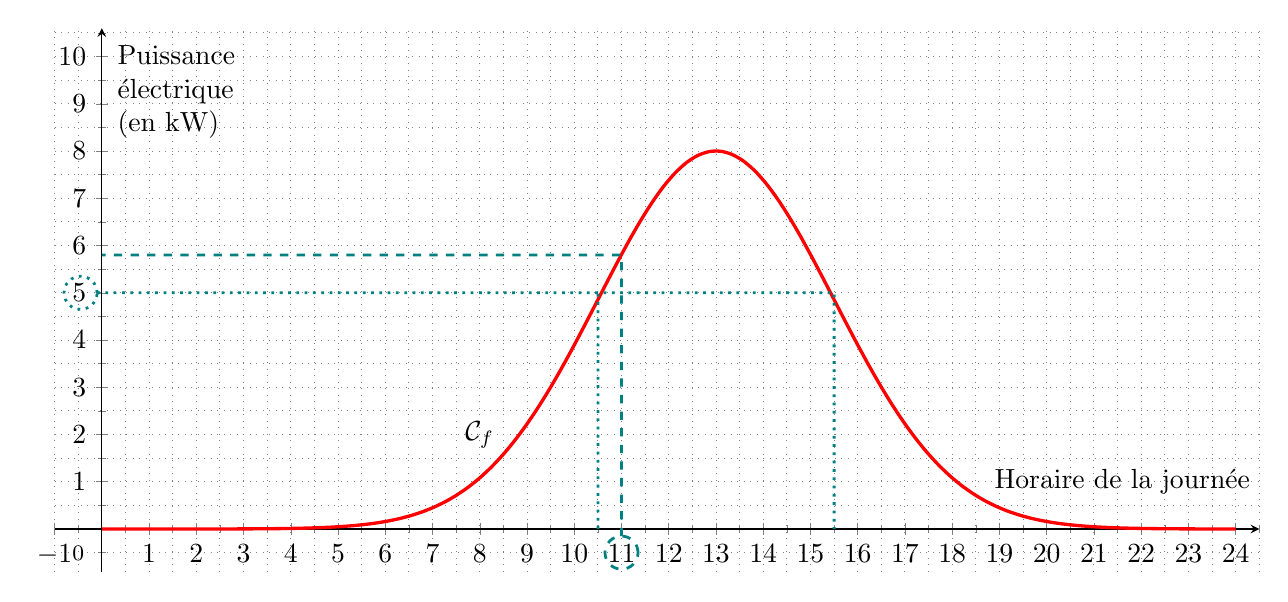
\begin{tikzpicture}
			\begin{axis}[/pgf/number format/.cd, use comma,
				x={6mm}, y={6mm},
				xmin = -1, xmax = 24.5,
				ymin = -0.9, ymax = 10.6,
				xtick distance=1,
				ytick distance=1,
				minor tick num = 1,
				grid=both, axis lines =center,
				grid style={gray!,line width=0.35pt,dotted}]
				\addplot[line width=1.2pt,color=red,smooth,samples=100,domain= 0:24] {8*exp(-0.08*(x-13)*(x-13))};
				\node[below left=1mm] at (axis cs: 0,0) {{\footnotesize 0}};
				\node at(axis cs: 8,2) {$ \mathcal{C}_f $};
				\node[text width=2cm] at(axis cs: 2,9.25) {Puissance électrique (en kW)};
				\node at(axis cs: 21.6,1) {Horaire de la journée};
				\draw[teal,dashed,line width=1pt] (axis cs: 11,-0.5) circle (0.35) (axis cs: 11,-0.15)--(axis cs: 11,5.8)--(axis cs: 0,5.8);
				\draw[teal,dotted,line width=1pt] (axis cs: -0.45,5) circle (0.35) (axis cs: -0.1,5)--(axis cs: 15.5,5)--(axis cs: 15.5,0) (axis cs: 10.5,0) -- (axis cs: 10.5,5);
			\end{axis}
		\end{tikzpicture}
	\end{center}

	
	
	
	
	
	
	
	
	
	
	
	
	
	\begin{enumerate}
		\item À $11$~h, la lecture graphique donne une puissance d'environ $5,75$~kW (à la précision permise par le graphique, voir le tracé en ligne tiretée).

		\item On lit les abscisses des points de la courbe situés de la droite d'équation $y=5$. (voir le tracé en ligne pointillée).
				On obtient approximativement :	\quad $f(x)\geqslant 5$ \quad pour $x\in[10,5 ; 15,5]$.

		\emph{Interprétation }: la puissance des panneaux solaires est supérieure ou égale à $5$~kW entre environ 10~h~30 et 15~h~30, soit pendant environ 5 heures dans la journée.
	\end{enumerate}

	\subsection*{Partie B}

	\begin{enumerate}
		\item Chaque année, le tarif augmente de $6~\%$ : on obtient le tarif d'une année en prenant le tarif de l'année précédente, multiplié par $1,06$.

		La suite $\left(c_{n}\right)$ est donc géométrique, de raison $q=1,06$ (et de premier terme $c_{0}=0,15$).

		\item Comme la suite est géométrique, pour tout entier naturel $n$ : \quad $c_{n}=c_{0}\times q^{\,n}=0,15\times 1,06^{\,n}$.

		\item L'année 2030 correspond à $2020 + 10$, donc $n=10$.

		Le coût pour $1$~kWh en 2030 est donc :\quad $c_{10}=0,15\times 1,06^{10}$.

		\item \begin{enumerate}
			\item \texttt{c} représente le coût (en euros) de $1$~kWh pour l'année considérée ($2020+n$) ;

			\texttt{S} représente l'économie totale cumulée (en euros) réalisée grâce aux panneaux solaires depuis 2020. Pour chaque exécution de la boucle \texttt{while}, on ajoute à la somme économisée précédemment la somme économisée cette année là, en multipliant la quantité d'énergie non achetée (\np[kWh]{2000}), par le prix d'achat. Puis, aux deux lignes suivantes, on met à jour l'indice de l'année, et le prix de l'énergie l'année suivante.

			\item Le programme affiche $16$ : il faut $16$ années pour que l'économie cumulée \texttt{S} dépasse \np{7000}~\euro{}, c'est-à-dire le coût d'installation.

			Selon cette modélisation, l'investissement de Camille sera rentabilisé au bout de $16$ ans, en 2020 + 16 = 2036.
		\end{enumerate}
	\end{enumerate}
